\documentclass[11pt,letterpaper]{article}
\usepackage{authblk} 
\usepackage{emnlp2017}
\usepackage{times}
\usepackage{url}
\usepackage{latexsym}
\usepackage[T1]{fontenc}    % use 8-bit T1 fonts
\usepackage{hyperref}       % hyperlinks
\usepackage{url}            % simple URL typesetting
\usepackage{booktabs}       % professional-quality tables
\usepackage{amsfonts}       % blackboard math symbols
\usepackage{nicefrac}       % compact symbols for 1/2, etc.
\usepackage{microtype}      % microtypography
\usepackage{amsmath}
\usepackage{mathtools}
\usepackage{graphicx,color,xcolor}
\usepackage{multirow}
\usepackage{enumitem} 
\usepackage{latexsym}
\usepackage{bm}
\usepackage{algorithm}
\usepackage[noend]{algpseudocode}

\usepackage{todonotes}

\graphicspath{{./figures}}

\usepackage{lipsum}

\newcommand\blfootnote[1]{%
  \begingroup
  \renewcommand\thefootnote{}\footnote{#1}%
  \addtocounter{footnote}{-1}%
  \endgroup
}


\DeclareMathOperator*{\argmax}{arg\,max}

% Uncomment this line for the final submission:
%\emnlpfinalcopy
%  Enter the EMNLP Paper ID here:
\def\emnlppaperid{***}

% To expand the titlebox for more authors, uncomment
% below and set accordingly.
% \addtolength\titlebox{.5in}    

\makeatletter
\def\BState{\State\hskip-\ALG@thistlm}
\makeatother
%\setlength\titlebox{5cm}
% You can expand the titlebox if you need extra space
% to show all the authors. Please do not make the titlebox
% smaller than 5cm (the original size); we will check this
% in the camera-ready version and ask you to change it back.

\newcommand\BibTeX{B{\sc ib}\TeX}
\def\NoNumber#1{{\def\alglinenumber##1{}\State #1}\addtocounter{ALG@line}{-1}}

\title{Enhancing Neural Machine Translation by\\ Searching Translation Memory}
\def \nyu{$^\ddag$}
\def \hku{$^\dagger$}
\def \cmu{$^\lozenge$}

\author[\hku]{\bf Jiatao Gu}
\author[\hku]{\bf Yong Wang}
\author[\nyu]{\bf Kyunghyun Cho}
\author[\hku]{\bf Victor O.K. Li}
\affil[\hku]{The University of Hong Kong}
\affil[\nyu]{New York University}
\affil[\hku]{\tt  \{jiataogu, wangyong, vli\}@eee.hku.hk}
\affil[\nyu]{\tt  kyunghyun.cho@nyu.edu}
\renewcommand\Authands{ and }
% \author{Jiatao Gu \\
%   University of Hong Kong \\
%   {\tt jiataogu@eee.hku.hk} \\\And
%   VictorO.K.Li \\
%   University of Hong Kong \\
%   {\tt vli@eee.hku.hk} \\\And
%   Kyunghyun Cho \\
%   Center for Data Science, and \\
%   Courant Institute of Mathematical Sciences, \\
%   New York University \\
%   {\tt kyunghyun.cho@nyu.edu} \\
%   }

\date{}

\begin{document}
\maketitle

\begin{abstract}
  This is an important problem\\
  This is an important problem\\  
  This is an important problem\\
  This is an important problem\\
  This is an important problem\\
  This is an important problem\\  
  This is an important problem\\
  This is an important problem\\
  This is an important problem\\
  This is an important problem\\
  This is an important problem\\  
  This is an important problem\\
  This is an important problem
\end{abstract}
\section{Introduction}
\begin{figure}[htbp]
\centering
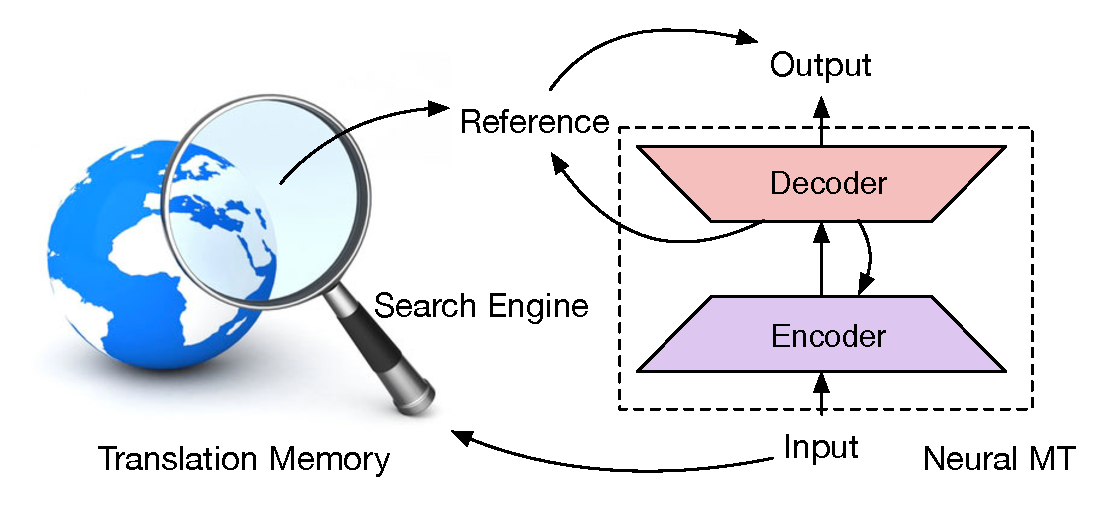
\includegraphics[width=0.98\linewidth]{figures/picture.pdf}
\caption{\label{fig.picture}A simple illustration}
\end{figure}

\section{Background}
\subsection{Neural Machine Translation}
Neural machine translation~\cite{sutskever2014sequence,bahdanau2014neural} is modeled as a conditional recurrent language model, where the source and target are sentences in two languages. Let us use $X=\left\{ x_1, \ldots, x_{T_s} \right\}$ and $Y=\left\{ y_1, \ldots, y_T \right\}$ to denote source and target sentences, respectively. Neural machine translation then models the target sentence given the source sentence as:
\begin{equation}
p(Y|X) = \prod_{t=1}^T p(y_t | y_{<t}, X).
\end{equation}
Each term on the r.h.s. of the equation above is modeled as a parametric function:
\begin{equation}
\label{eq.prob}
p(y_t|y_{<t}, X)\propto \exp\left(g\left(y_t, z_t; \theta_g\right)\right),
\end{equation}
where 
%\begin{align*}
$z_t = f(z_{t-1}, y_{t-1}, c_t(X; \theta_e); \theta_f)$.
%\end{align*}
$f$ is a recurrent function that compresses all the previous target words $y_{<t}$ and the time-dependent representation (or called context) $c_t(X; \theta_e)$ of the source sentence $X$ into the decoder state $z_t$. $g$ is a read-out function that transforms $z_t$ into the distribution over a fixed vocabulary.  Here, we use $\theta = \{\theta_e, \theta_f, \theta_g\}$ as the parameters of the neural MT system.
\paragraph{Attention Mechanism}
In default, $c_t(X)$ is implemented as a bidirectional recurrent network encoder of the source sentence coupled with an attention mechanism. We use $h_\tau$ as the concatenation of the states produced by the backward and forward encoder for each input word $x_\tau$, and compute the context as the weighted sum of the encoder states,
\begin{equation}
\label{eq.attention}
c_t = \sum_{\tau=1}^{T_s}\alpha_{t\tau}h_\tau
\end{equation}
where $\alpha_{t\tau} \propto \exp\left[\phi_{att}\left(h_\tau, z_{t-1}\right)\right]$ are the attention weights, and $\phi_{att}$ is a scoring function. Naturally, the attention summarizes the relatedness between the source words and the target translation, which indicates the context vector $c_t$ has a identity correspondence to the target word $y_t$, as shown in Fig.~\ref{fig.nmt}, 
\begin{figure}[htbp]
\centering
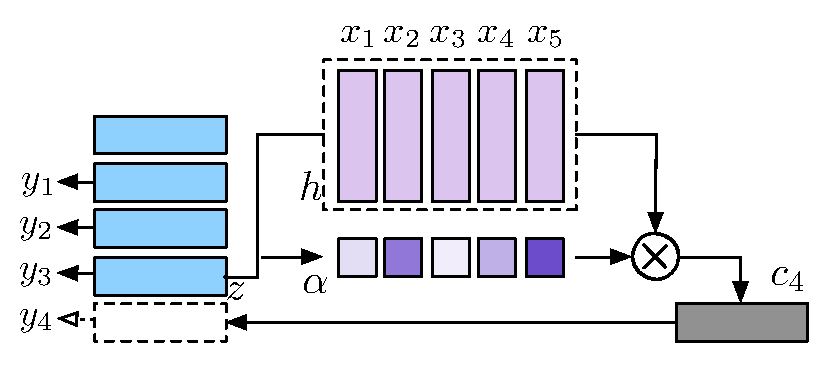
\includegraphics[width=0.85\linewidth]{figures/nmt1.pdf}
\caption{\label{fig.nmt}An illustration for the attention mechanism of a standard Neural MT model.  }
\end{figure}

The whole neural MT model can be trained end-to-end by maximizing the log-probability of a reference translation given a source sentence. For testing, search-based methods, such as Beam-search are usually applied to find a proper translation.
\subsection{Translation Memory}
Typically, the Translation Memory (TM) refers to a computer aided translation tool for professional translators.
It is very different research field, has been proven that the combination of TM~\cite{li2016phrase} will also benefit the translation quality of a machine translation system.

Generally speaking, what we call as ``Translation Memory'' means anything that stores raw translation knowledge (e.g. translation pairs, phrase tables, e.t.c.), and can be retrieved through a search engine. Naturally, a translation memory has no limits, and can be accumulated from the history human translation records. In practice, in terms of the storage limitation, it usually impossible get exactly the same translation by searching the memory. 


\section{Translation Memory Enhanced Neural Machine Translation (TM-NMT)}
%The basic concept of this paper is that: teaching a Neural MT system to search similar translation examples from TM, and based on the retrieved examples and its own knowledge to generate better translation.
\subsection{Problem Definition}
Given a neural MT system and a large scale translation memory database, we are interested in making the MT system to automatically search relevant translation pairs from the translation memory with a search engine, and then to use these information to enhance the translation quality. 

We can summarize our model into two phases: the \textit{searching phase} and the \textit{translation phase}.
Suppose we want to translate from the source sentence $X$ to the target sentence $Y$. We will first apply $X$ as a query to a search engine, and receive the answer translation pairs $(X', Y')$\footnote{For simplicity, we only discuss one answer in the definition. However, it can be trivially extended to multiple answers.}. The learning objective is to maximize the log-likelihood conditioning on both the source sentence and the memorized translation pairs, as follows:
\begin{equation}
\left\{
\begin{array}{r@{\;=\;}l}
X', Y' & F_{ss}(X, \mathcal{M})\\
\max L_\phi & \log p_\phi(Y|X, X', Y')
\end{array}
\right.
\end{equation}
where we use $F_{ss}$ as a search engine, and $\mathcal{M}$ as the translation memory. Note that the source $X$ is not necessarily included in $\mathcal{M}$. We use $\phi$ as the parameters of a TM-enhanced Neural MT model, which will be discussed in detail in later sections.
\subsection{Searching Phase}
In this section, we discuss about the method using search engine to retrieve similar translation pairs from the translation memory $\mathcal{M}$, which is a set of translated source-target pairs. The search engine accepts the source sentence $X$ as a query, and returns the best match $X'$ by comparing the similarity over all the source sentences stored in $\mathcal{M}$ using a similarity function $s(X, X')$. As shown in Fig.~\ref{fig.search}, the corresponded translation $Y'$ is returned simultaneously.
\begin{figure}[htbp]
\centering
\vspace{-8pt}
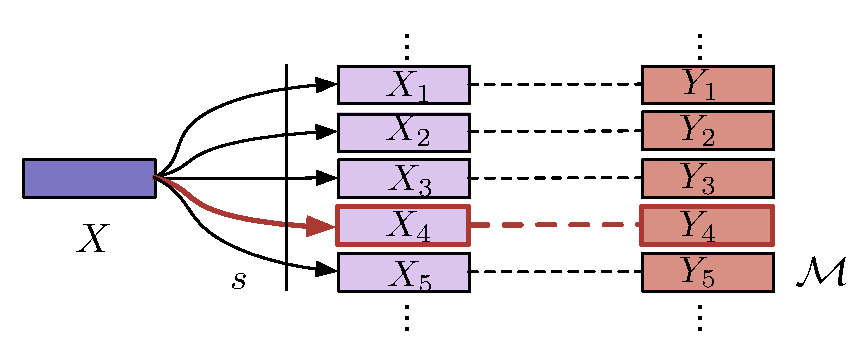
\includegraphics[width=0.85\linewidth]{figures/search.pdf}
\vspace{-5pt}
\caption{\label{fig.search}An illustration for the Similarity-based Search. Each block represents a sentence.}
\vspace{-8pt}
\end{figure}
\paragraph{Choice of $s$}
It depends on what level of the information we adopt, which can be either lexical-level matching scores (count-vector cosine-similarity, Edit-distance, BLEU, etc.) or the semantically relatedness computed by a neural network~\cite{hu2014convolutional}. However, as human searches the related translation examples to help doing translation, it is more natural to match shallow features of language usage other than understanding the semantic meanings of sentences. Considering on this, we use two types of non-parameterized metrics in our experiments: the edit distance $s_{edit}$ and the BLEU score $s_{bleu}$. Following the previous work~\cite{li2016phrase}, we also constrain $s_{edit}\in[0, 1]$ by defining the fuzzy matching score as follows:
\begin{equation}
s_{fuzzy}(X, X') = 1 - \frac{s_{edit}(X, X')}{\max\left(|X|, |X'|\right)}
\end{equation}
Both the metrics are not trainable and sub-optimal, however, they are efficiently enough to apply on a large translation memory. 
Alternatively, it is possible to design a light-weight similarity function to select the best reference pair with REINFORCE~\cite{williams1992simple}, while we leave this part in future work, and leverage the learning load to the translation phase.
\paragraph{Speed-up} The computational complexity is still linear to the size of the translation memory, which makes the searching painful even with the edit distance. An optional approximation is first using a rough inverse-indexing based search engine to collect a subset of the translation memory $\tilde{\mathcal{M}}\subseteq \mathcal{M}$, and then applying more accurate metrics on it. It makes the framework scalable on a large training set with a large translation memory. 
\begin{figure*}[htpb]
\label{framework}
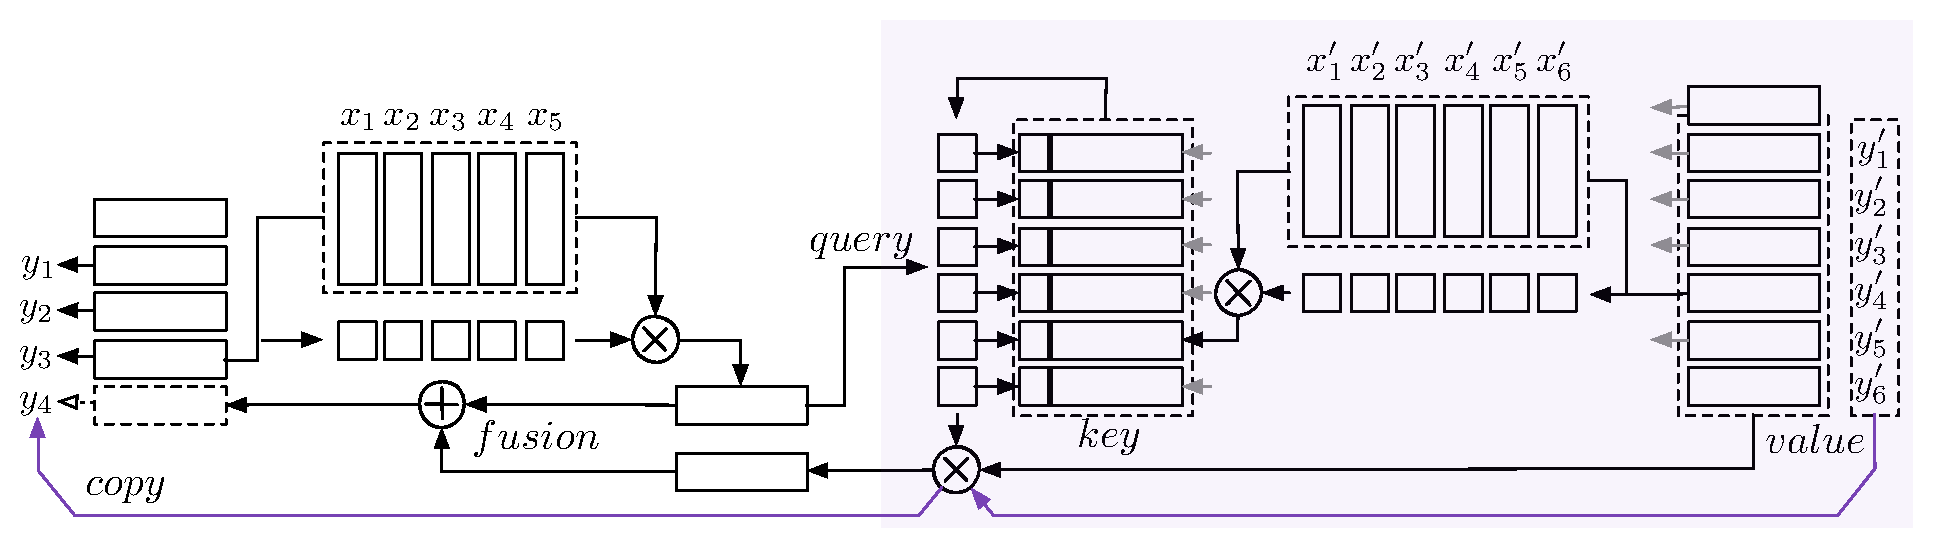
\includegraphics[width=\linewidth]{figures/framework1.pdf}
\caption{\label{fig.tmnmt}The whole architecture of the proposed TM-NMT model}
\end{figure*}

\paragraph{Return}
As for the return of searching phase, it is possible to simply pick the Top-1 match of the similarity score, i,e. $(X', Y')=\arg\max_{X'}s(X, X')$.  To obtain more information from $\mathcal{M}$, we can trivially extend to return multiple pairs by choosing the Top-K candidates which, however, is not efficient as the Top-K matches of the similarity function usually contains much redundancy.
A heuristic algorithm here

\subsection{Translation Phase}
The standard Attention-based Neural MT model is modified to incorporate the retrieved translation pairs into translation. 
\paragraph{Challenges}
When translating words given $X$ and $X', Y'$, a natural flow of ``attention'' will go through $X \xrightarrow{\nearrow X'^{\rightarrow}Y' \searrow} Y$ so that the model knows ``where and how the source words can be translated in the example'' and merges that information with the original Neural MT system. One closely related topic is \textit{Copying Mechanism}~\cite{gu2016incorporating,gulcehre2016pointing}, which can be easily extend to our problem by allowing \textit{copying} from $Y'$ to $Y$. Different from the existing models which is a \textit{one-step matching}  from the source words (or associated rare words) to the target side,  what in our case requires using $X$ to match $X'$ (keys) , but choosing the most proper words from $Y'$ (values).  Therefore, we need to solve a problem of \textit{multi-step matching} as both $X \& Y$ and $X' \& Y'$ typically do not have clear alignments, making the modelling and computation complicated.

On the other hand, due to the data sparsity, the memory $\mathcal{M}$ cannot make sure always return the most desired translation pairs for the model to look at. Thus, the design of the translation model should be flexible so that the bad memory information will break down the original translation model. As shown in Fig.~\ref{fig.tmnmt}, we propose the TM-NMT model  targeting on these challenges as following steps. 
\paragraph{Dynamic Key Generation}
Firstly, we  run a separate Neural MT model $\theta'$ over $Y'$, given $X'$ as the source sentence , and collect the context vector for each target word $y'\in Y'$ following the attention mechanism in Eq.~\ref{eq.attention}. The generated context vectors are stored as keys before translation starts.  We use $c'_t$ to denote the key associated with $y'_t$.  
In the same way with Eq.~\ref{eq.attention}, we can also generate the key $c_t$  for translating $y_t$ using the current translation model $\theta$, which can be further used for matching. Note here we mentioned to use two Neural MT models ($\theta$, $\theta'$), and in practise we use $\theta=\theta'$.

Generating context vectors from attention mechanism as keys is reasonable for some reasons. Most importantly,  $c_t (c'_t)$ is the weighted sum of the hidden states of the source words encoder, and is explained as the attention result to produce the target word $y_t (y'_t)$, which nicely fits our intention to use the source information as keys, in the meantime, transforms the problem into \textit{one-step matching}.  As we can pre-compute and store the keys offline for each target word in the translation memory, we can still keep the on-line translation relatively efficient even with a large memory.
% we can easily extend this method to multiple-memory setting by stacking the pre-computed ``key-target" pairs together without effecting the on-line translation speed too much.

\paragraph{Matching} 
The matching scores of the query $c_t$ and memory keys $\{c'_t\}_{t=1}^{T'}$ consider the two things:
\begin{itemize}
	\vspace{-5pt}
	\item Similarity: inner product
	\vspace{-5pt}
	\item Coverage: as discussed in \cite{tu2016modeling}, we also noticed that
	\vspace{-5pt}
\end{itemize}
Thus, we propose the matching function as
\begin{equation}
\begin{split}
	&E_{\psi}(c_t, c'_\tau) = c_t^TMc'_\tau - \lambda \beta_t\\
	&q_{t, \tau}  = \frac{\exp(E_{\psi}(c_t, c'_\tau)/\eta)}{\sum_{\tau'} \exp(E_{\psi}(c_t, c'_{\tau'})/\eta)}
\end{split}
\end{equation}
where  $\beta_t$ is the cumulative coverage term. To keep the translation phase differentiable for end-to-end training, we use a ``soft match" as $q_{t,\tau}$, where $\eta \geq 1$ is the temperature to control the distribution. 

\paragraph{Incorporation} Once we obtain the a matching result between the query $c_t$ and the retrieved translation pair, it is possible to use the matched information to help the current translation. In our implementation, two modes are designed to incorporate the information of memory into translation:
\begin{itemize}
	\vspace{-5pt}
	\item \textbf{copy mode}: we directly use the ``soft-match" as $q_{t,\tau}=p_{\text{copy}}(y_t =y'_\tau)$ over the target words. Obviously, $p_{\text{copy}}(y) = 0, \forall y \notin Y'$. Thus we rewrite the output probability as:
	\begin{equation}
	\label{eq.copy}
		p(y_t|\cdot) = \zeta_t \cdot p_{\text{copy}} + (1 -\zeta_t) \cdot p_{\text{gen}}   
	\end{equation}
	where $p_{\text{gen}}$ is denoted as the distribution of the original Neural MT model (Eq.~\ref{eq.prob}).
	\vspace{-5pt}
	\item \textbf{fusion mode}: we can also use a fusion model by treating the ``soft-match" as the weights over the decoder states of the TM target words, that is, 
	%\begin{equation}
		$\tilde{z}_t = \sum_{\tau=1}^{T'} q_{t, \tau} \cdot z'_\tau$, and compute the weighted hidden state together with the state $z_t$ of the original model:
		\begin{equation}
		\label{eq.fusion}
		z_{\text{fusion}} = \zeta_t \cdot \tilde{z}_t + (1 -\zeta_t) \cdot z_t 
		\end{equation}
where we use the fused state $z_{\text{fusion}}$ to replace $z_t$ in Eq.~\ref{eq.prob} to get the output distribution.	
\vspace{-5pt}
\end{itemize}
Both the 	``copy mode" and the ``fusion mode" are trying to bias the original distribution with the information from translation memory. However, they work in very different ways. 
\paragraph{Gating} It is also notable that in both Eq.~\ref{eq.copy} and~\ref{eq.fusion}, an additional scalar $\zeta_t \in [0, 1]$ is used as a gate to control the information flow between the original Neural MT system and the translation memory. In our implementation, the gate is computed by a neural network $\zeta_t = f_{\text{gate}}(c_t, z_t, \tilde{z}_t)$, with both $z_t$ and $\tilde{z}_t$ in the input. In this way, the gate is supposed to be closed ($=0$) if the retrieved memory does not contain any useful information. In such case, the model will use the original model for translation; In contrast, 


\subsection{Discussion}
\begin{itemize}
\item \textbf{Long term memory}~ plain text, never forgetting, e.g. translation memory
\item \textbf{Short term memory}~ example-level, hybrid representation
\item \textbf{Instantaneous memory}~ word-level, coverage
\end{itemize}


\section{Experiments}
\subsection{Experimental Setting}
\paragraph{Data} Two sources of public available dataset are used in our experiments: JRC-Acquis Corpus\footnote{http://optima.jrc.it/Acquis/JRC-Acquis.3.0/corpus/} and WMT-15

\section*{Acknowledgments}

Do not number the acknowledgment section.

\bibliography{emnlp2017}
\bibliographystyle{emnlp_natbib}

\end{document}
